% Generated by ArticleSignalDiagrams. Opaque vector fills only.
\documentclass[10pt,tikz,border=5pt]{standalone}
\usepackage{lmodern}
\usetikzlibrary{fit}
\begin{document}
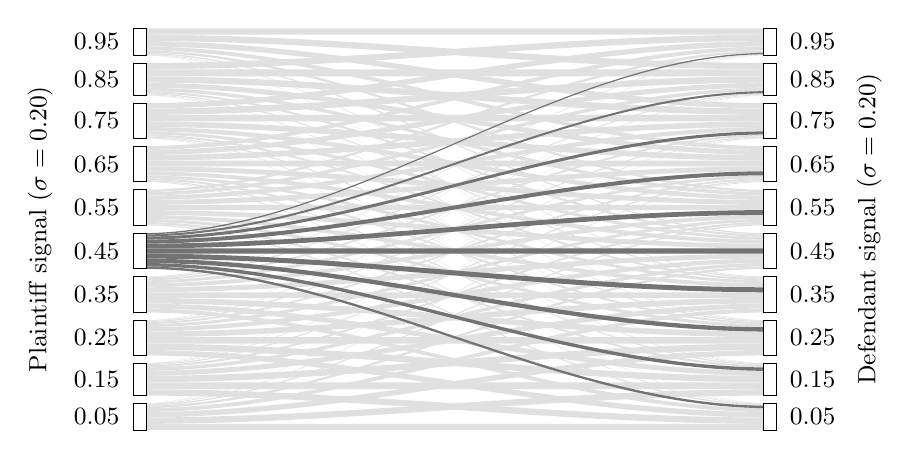
\begin{tikzpicture}[x=1cm,y=1cm,font=\small]\path[fill=black!12,draw=none] (3.3,-5.1) .. controls (6,-5.1) and (8.6,-5.1) .. (11.3,-5.1) -- (11.3,-5.021463) .. controls (8.6,-5.021463) and (6,-5.021463) .. (3.3,-5.021463) -- cycle;
\path[fill=black!12,draw=none] (3.3,-5.021463) .. controls (6,-5.021463) and (8.6,-4.662119) .. (11.3,-4.662119) -- (11.3,-4.581248) .. controls (8.6,-4.581248) and (6,-4.940592) .. (3.3,-4.940592) -- cycle;
\path[fill=black!12,draw=none] (3.3,-4.940592) .. controls (6,-4.940592) and (8.6,-4.151878) .. (11.3,-4.151878) -- (11.3,-4.082869) .. controls (8.6,-4.082869) and (6,-4.871582) .. (3.3,-4.871582) -- cycle;
\path[fill=black!12,draw=none] (3.3,-4.871582) .. controls (6,-4.871582) and (8.6,-3.605927) .. (11.3,-3.605927) -- (11.3,-3.55635) .. controls (8.6,-3.55635) and (6,-4.822005) .. (3.3,-4.822005) -- cycle;
\path[fill=black!12,draw=none] (3.3,-4.822005) .. controls (6,-4.822005) and (8.6,-3.051926) .. (11.3,-3.051926) -- (11.3,-3.021394) .. controls (8.6,-3.021394) and (6,-4.791473) .. (3.3,-4.791473) -- cycle;
\path[fill=black!12,draw=none] (3.3,-4.791473) .. controls (6,-4.791473) and (8.6,-2.5) .. (11.3,-2.5) -- (11.3,-2.483581) .. controls (8.6,-2.483581) and (6,-4.775054) .. (3.3,-4.775054) -- cycle;
\path[fill=black!12,draw=none] (3.3,-4.775054) .. controls (6,-4.775054) and (8.6,-1.948074) .. (11.3,-1.948074) -- (11.3,-1.94024) .. controls (8.6,-1.94024) and (6,-4.76722) .. (3.3,-4.76722) -- cycle;
\path[fill=black!12,draw=none] (3.3,-4.76722) .. controls (6,-4.76722) and (8.6,-1.394073) .. (11.3,-1.394073) -- (11.3,-1.39072) .. controls (8.6,-1.39072) and (6,-4.763866) .. (3.3,-4.763866) -- cycle;
\path[fill=black!12,draw=none] (3.3,-4.763866) .. controls (6,-4.763866) and (8.6,-0.848122) .. (11.3,-0.848122) -- (11.3,-0.846827) .. controls (8.6,-0.846827) and (6,-4.762571) .. (3.3,-4.762571) -- cycle;
\path[fill=black!12,draw=none] (3.3,-4.762571) .. controls (6,-4.762571) and (8.6,-0.337881) .. (11.3,-0.337881) -- (11.3,-0.337429) .. controls (8.6,-0.337429) and (6,-4.762119) .. (3.3,-4.762119) -- cycle;
\path[fill=black!12,draw=none] (3.3,-4.662119) .. controls (6,-4.662119) and (8.6,-5.021463) .. (11.3,-5.021463) -- (11.3,-4.940592) .. controls (8.6,-4.940592) and (6,-4.581248) .. (3.3,-4.581248) -- cycle;
\path[fill=black!12,draw=none] (3.3,-4.581248) .. controls (6,-4.581248) and (8.6,-4.581248) .. (11.3,-4.581248) -- (11.3,-4.493092) .. controls (8.6,-4.493092) and (6,-4.493092) .. (3.3,-4.493092) -- cycle;
\path[fill=black!12,draw=none] (3.3,-4.493092) .. controls (6,-4.493092) and (8.6,-4.082869) .. (11.3,-4.082869) -- (11.3,-4.001965) .. controls (8.6,-4.001965) and (6,-4.412189) .. (3.3,-4.412189) -- cycle;
\path[fill=black!12,draw=none] (3.3,-4.412189) .. controls (6,-4.412189) and (8.6,-3.55635) .. (11.3,-3.55635) -- (11.3,-3.492698) .. controls (8.6,-3.492698) and (6,-4.348537) .. (3.3,-4.348537) -- cycle;
\path[fill=black!12,draw=none] (3.3,-4.348537) .. controls (6,-4.348537) and (8.6,-3.021394) .. (11.3,-3.021394) -- (11.3,-2.977664) .. controls (8.6,-2.977664) and (6,-4.304808) .. (3.3,-4.304808) -- cycle;
\path[fill=black!12,draw=none] (3.3,-4.304808) .. controls (6,-4.304808) and (8.6,-2.483581) .. (11.3,-2.483581) -- (11.3,-2.456925) .. controls (8.6,-2.456925) and (6,-4.278152) .. (3.3,-4.278152) -- cycle;
\path[fill=black!12,draw=none] (3.3,-4.278152) .. controls (6,-4.278152) and (8.6,-1.94024) .. (11.3,-1.94024) -- (11.3,-1.925663) .. controls (8.6,-1.925663) and (6,-4.263576) .. (3.3,-4.263576) -- cycle;
\path[fill=black!12,draw=none] (3.3,-4.263576) .. controls (6,-4.263576) and (8.6,-1.39072) .. (11.3,-1.39072) -- (11.3,-1.383527) .. controls (8.6,-1.383527) and (6,-4.256383) .. (3.3,-4.256383) -- cycle;
\path[fill=black!12,draw=none] (3.3,-4.256383) .. controls (6,-4.256383) and (8.6,-0.846827) .. (11.3,-0.846827) -- (11.3,-0.843617) .. controls (8.6,-0.843617) and (6,-4.253173) .. (3.3,-4.253173) -- cycle;
\path[fill=black!12,draw=none] (3.3,-4.253173) .. controls (6,-4.253173) and (8.6,-0.337429) .. (11.3,-0.337429) -- (11.3,-0.336134) .. controls (8.6,-0.336134) and (6,-4.251878) .. (3.3,-4.251878) -- cycle;
\path[fill=black!12,draw=none] (3.3,-4.151878) .. controls (6,-4.151878) and (8.6,-4.940592) .. (11.3,-4.940592) -- (11.3,-4.871582) .. controls (8.6,-4.871582) and (6,-4.082869) .. (3.3,-4.082869) -- cycle;
\path[fill=black!12,draw=none] (3.3,-4.082869) .. controls (6,-4.082869) and (8.6,-4.493092) .. (11.3,-4.493092) -- (11.3,-4.412189) .. controls (8.6,-4.412189) and (6,-4.001965) .. (3.3,-4.001965) -- cycle;
\path[fill=black!12,draw=none] (3.3,-4.001965) .. controls (6,-4.001965) and (8.6,-4.001965) .. (11.3,-4.001965) -- (11.3,-3.920654) .. controls (8.6,-3.920654) and (6,-3.920654) .. (3.3,-3.920654) -- cycle;
\path[fill=black!12,draw=none] (3.3,-3.920654) .. controls (6,-3.920654) and (8.6,-3.492698) .. (11.3,-3.492698) -- (11.3,-3.421336) .. controls (8.6,-3.421336) and (6,-3.849292) .. (3.3,-3.849292) -- cycle;
\path[fill=black!12,draw=none] (3.3,-3.849292) .. controls (6,-3.849292) and (8.6,-2.977664) .. (11.3,-2.977664) -- (11.3,-2.922094) .. controls (8.6,-2.922094) and (6,-3.793721) .. (3.3,-3.793721) -- cycle;
\path[fill=black!12,draw=none] (3.3,-3.793721) .. controls (6,-3.793721) and (8.6,-2.456925) .. (11.3,-2.456925) -- (11.3,-2.418102) .. controls (8.6,-2.418102) and (6,-3.754898) .. (3.3,-3.754898) -- cycle;
\path[fill=black!12,draw=none] (3.3,-3.754898) .. controls (6,-3.754898) and (8.6,-1.925663) .. (11.3,-1.925663) -- (11.3,-1.901189) .. controls (8.6,-1.901189) and (6,-3.730424) .. (3.3,-3.730424) -- cycle;
\path[fill=black!12,draw=none] (3.3,-3.730424) .. controls (6,-3.730424) and (8.6,-1.383527) .. (11.3,-1.383527) -- (11.3,-1.369576) .. controls (8.6,-1.369576) and (6,-3.716473) .. (3.3,-3.716473) -- cycle;
\path[fill=black!12,draw=none] (3.3,-3.716473) .. controls (6,-3.716473) and (8.6,-0.843617) .. (11.3,-0.843617) -- (11.3,-0.836424) .. controls (8.6,-0.836424) and (6,-3.70928) .. (3.3,-3.70928) -- cycle;
\path[fill=black!12,draw=none] (3.3,-3.70928) .. controls (6,-3.70928) and (8.6,-0.336134) .. (11.3,-0.336134) -- (11.3,-0.33278) .. controls (8.6,-0.33278) and (6,-3.705927) .. (3.3,-3.705927) -- cycle;
\path[fill=black!12,draw=none] (3.3,-3.605927) .. controls (6,-3.605927) and (8.6,-4.871582) .. (11.3,-4.871582) -- (11.3,-4.822005) .. controls (8.6,-4.822005) and (6,-3.55635) .. (3.3,-3.55635) -- cycle;
\path[fill=black!12,draw=none] (3.3,-3.55635) .. controls (6,-3.55635) and (8.6,-4.412189) .. (11.3,-4.412189) -- (11.3,-4.348537) .. controls (8.6,-4.348537) and (6,-3.492698) .. (3.3,-3.492698) -- cycle;
\path[fill=black!12,draw=none] (3.3,-3.492698) .. controls (6,-3.492698) and (8.6,-3.920654) .. (11.3,-3.920654) -- (11.3,-3.849292) .. controls (8.6,-3.849292) and (6,-3.421336) .. (3.3,-3.421336) -- cycle;
\path[fill=black!12,draw=none] (3.3,-3.421336) .. controls (6,-3.421336) and (8.6,-3.421336) .. (11.3,-3.421336) -- (11.3,-3.350347) .. controls (8.6,-3.350347) and (6,-3.350347) .. (3.3,-3.350347) -- cycle;
\path[fill=black!12,draw=none] (3.3,-3.350347) .. controls (6,-3.350347) and (8.6,-2.922094) .. (11.3,-2.922094) -- (11.3,-2.858738) .. controls (8.6,-2.858738) and (6,-3.286991) .. (3.3,-3.286991) -- cycle;
\path[fill=black!12,draw=none] (3.3,-3.286991) .. controls (6,-3.286991) and (8.6,-2.418102) .. (11.3,-2.418102) -- (11.3,-2.367079) .. controls (8.6,-2.367079) and (6,-3.235967) .. (3.3,-3.235967) -- cycle;
\path[fill=black!12,draw=none] (3.3,-3.235967) .. controls (6,-3.235967) and (8.6,-1.901189) .. (11.3,-1.901189) -- (11.3,-1.864033) .. controls (8.6,-1.864033) and (6,-3.198811) .. (3.3,-3.198811) -- cycle;
\path[fill=black!12,draw=none] (3.3,-3.198811) .. controls (6,-3.198811) and (8.6,-1.369576) .. (11.3,-1.369576) -- (11.3,-1.345102) .. controls (8.6,-1.345102) and (6,-3.174337) .. (3.3,-3.174337) -- cycle;
\path[fill=black!12,draw=none] (3.3,-3.174337) .. controls (6,-3.174337) and (8.6,-0.836424) .. (11.3,-0.836424) -- (11.3,-0.821848) .. controls (8.6,-0.821848) and (6,-3.15976) .. (3.3,-3.15976) -- cycle;
\path[fill=black!12,draw=none] (3.3,-3.15976) .. controls (6,-3.15976) and (8.6,-0.33278) .. (11.3,-0.33278) -- (11.3,-0.324946) .. controls (8.6,-0.324946) and (6,-3.151926) .. (3.3,-3.151926) -- cycle;
\path[fill=black!12,draw=none] (3.3,-2.5) .. controls (6,-2.5) and (8.6,-4.791473) .. (11.3,-4.791473) -- (11.3,-4.775054) .. controls (8.6,-4.775054) and (6,-2.483581) .. (3.3,-2.483581) -- cycle;
\path[fill=black!12,draw=none] (3.3,-2.483581) .. controls (6,-2.483581) and (8.6,-4.304808) .. (11.3,-4.304808) -- (11.3,-4.278152) .. controls (8.6,-4.278152) and (6,-2.456925) .. (3.3,-2.456925) -- cycle;
\path[fill=black!12,draw=none] (3.3,-2.456925) .. controls (6,-2.456925) and (8.6,-3.793721) .. (11.3,-3.793721) -- (11.3,-3.754898) .. controls (8.6,-3.754898) and (6,-2.418102) .. (3.3,-2.418102) -- cycle;
\path[fill=black!12,draw=none] (3.3,-2.418102) .. controls (6,-2.418102) and (8.6,-3.286991) .. (11.3,-3.286991) -- (11.3,-3.235967) .. controls (8.6,-3.235967) and (6,-2.367079) .. (3.3,-2.367079) -- cycle;
\path[fill=black!12,draw=none] (3.3,-2.367079) .. controls (6,-2.367079) and (8.6,-2.793557) .. (11.3,-2.793557) -- (11.3,-2.732921) .. controls (8.6,-2.732921) and (6,-2.306443) .. (3.3,-2.306443) -- cycle;
\path[fill=black!12,draw=none] (3.3,-2.306443) .. controls (6,-2.306443) and (8.6,-2.306443) .. (11.3,-2.306443) -- (11.3,-2.241262) .. controls (8.6,-2.241262) and (6,-2.241262) .. (3.3,-2.241262) -- cycle;
\path[fill=black!12,draw=none] (3.3,-2.241262) .. controls (6,-2.241262) and (8.6,-1.813009) .. (11.3,-1.813009) -- (11.3,-1.749653) .. controls (8.6,-1.749653) and (6,-2.177906) .. (3.3,-2.177906) -- cycle;
\path[fill=black!12,draw=none] (3.3,-2.177906) .. controls (6,-2.177906) and (8.6,-1.306279) .. (11.3,-1.306279) -- (11.3,-1.250708) .. controls (8.6,-1.250708) and (6,-2.122336) .. (3.3,-2.122336) -- cycle;
\path[fill=black!12,draw=none] (3.3,-2.122336) .. controls (6,-2.122336) and (8.6,-0.795192) .. (11.3,-0.795192) -- (11.3,-0.751463) .. controls (8.6,-0.751463) and (6,-2.078606) .. (3.3,-2.078606) -- cycle;
\path[fill=black!12,draw=none] (3.3,-2.078606) .. controls (6,-2.078606) and (8.6,-0.308527) .. (11.3,-0.308527) -- (11.3,-0.277995) .. controls (8.6,-0.277995) and (6,-2.048074) .. (3.3,-2.048074) -- cycle;
\path[fill=black!12,draw=none] (3.3,-1.948074) .. controls (6,-1.948074) and (8.6,-4.775054) .. (11.3,-4.775054) -- (11.3,-4.76722) .. controls (8.6,-4.76722) and (6,-1.94024) .. (3.3,-1.94024) -- cycle;
\path[fill=black!12,draw=none] (3.3,-1.94024) .. controls (6,-1.94024) and (8.6,-4.278152) .. (11.3,-4.278152) -- (11.3,-4.263576) .. controls (8.6,-4.263576) and (6,-1.925663) .. (3.3,-1.925663) -- cycle;
\path[fill=black!12,draw=none] (3.3,-1.925663) .. controls (6,-1.925663) and (8.6,-3.754898) .. (11.3,-3.754898) -- (11.3,-3.730424) .. controls (8.6,-3.730424) and (6,-1.901189) .. (3.3,-1.901189) -- cycle;
\path[fill=black!12,draw=none] (3.3,-1.901189) .. controls (6,-1.901189) and (8.6,-3.235967) .. (11.3,-3.235967) -- (11.3,-3.198811) .. controls (8.6,-3.198811) and (6,-1.864033) .. (3.3,-1.864033) -- cycle;
\path[fill=black!12,draw=none] (3.3,-1.864033) .. controls (6,-1.864033) and (8.6,-2.732921) .. (11.3,-2.732921) -- (11.3,-2.681898) .. controls (8.6,-2.681898) and (6,-1.813009) .. (3.3,-1.813009) -- cycle;
\path[fill=black!12,draw=none] (3.3,-1.813009) .. controls (6,-1.813009) and (8.6,-2.241262) .. (11.3,-2.241262) -- (11.3,-2.177906) .. controls (8.6,-2.177906) and (6,-1.749653) .. (3.3,-1.749653) -- cycle;
\path[fill=black!12,draw=none] (3.3,-1.749653) .. controls (6,-1.749653) and (8.6,-1.749653) .. (11.3,-1.749653) -- (11.3,-1.678664) .. controls (8.6,-1.678664) and (6,-1.678664) .. (3.3,-1.678664) -- cycle;
\path[fill=black!12,draw=none] (3.3,-1.678664) .. controls (6,-1.678664) and (8.6,-1.250708) .. (11.3,-1.250708) -- (11.3,-1.179346) .. controls (8.6,-1.179346) and (6,-1.607302) .. (3.3,-1.607302) -- cycle;
\path[fill=black!12,draw=none] (3.3,-1.607302) .. controls (6,-1.607302) and (8.6,-0.751463) .. (11.3,-0.751463) -- (11.3,-0.687811) .. controls (8.6,-0.687811) and (6,-1.54365) .. (3.3,-1.54365) -- cycle;
\path[fill=black!12,draw=none] (3.3,-1.54365) .. controls (6,-1.54365) and (8.6,-0.277995) .. (11.3,-0.277995) -- (11.3,-0.228418) .. controls (8.6,-0.228418) and (6,-1.494073) .. (3.3,-1.494073) -- cycle;
\path[fill=black!12,draw=none] (3.3,-1.394073) .. controls (6,-1.394073) and (8.6,-4.76722) .. (11.3,-4.76722) -- (11.3,-4.763866) .. controls (8.6,-4.763866) and (6,-1.39072) .. (3.3,-1.39072) -- cycle;
\path[fill=black!12,draw=none] (3.3,-1.39072) .. controls (6,-1.39072) and (8.6,-4.263576) .. (11.3,-4.263576) -- (11.3,-4.256383) .. controls (8.6,-4.256383) and (6,-1.383527) .. (3.3,-1.383527) -- cycle;
\path[fill=black!12,draw=none] (3.3,-1.383527) .. controls (6,-1.383527) and (8.6,-3.730424) .. (11.3,-3.730424) -- (11.3,-3.716473) .. controls (8.6,-3.716473) and (6,-1.369576) .. (3.3,-1.369576) -- cycle;
\path[fill=black!12,draw=none] (3.3,-1.369576) .. controls (6,-1.369576) and (8.6,-3.198811) .. (11.3,-3.198811) -- (11.3,-3.174337) .. controls (8.6,-3.174337) and (6,-1.345102) .. (3.3,-1.345102) -- cycle;
\path[fill=black!12,draw=none] (3.3,-1.345102) .. controls (6,-1.345102) and (8.6,-2.681898) .. (11.3,-2.681898) -- (11.3,-2.643075) .. controls (8.6,-2.643075) and (6,-1.306279) .. (3.3,-1.306279) -- cycle;
\path[fill=black!12,draw=none] (3.3,-1.306279) .. controls (6,-1.306279) and (8.6,-2.177906) .. (11.3,-2.177906) -- (11.3,-2.122336) .. controls (8.6,-2.122336) and (6,-1.250708) .. (3.3,-1.250708) -- cycle;
\path[fill=black!12,draw=none] (3.3,-1.250708) .. controls (6,-1.250708) and (8.6,-1.678664) .. (11.3,-1.678664) -- (11.3,-1.607302) .. controls (8.6,-1.607302) and (6,-1.179346) .. (3.3,-1.179346) -- cycle;
\path[fill=black!12,draw=none] (3.3,-1.179346) .. controls (6,-1.179346) and (8.6,-1.179346) .. (11.3,-1.179346) -- (11.3,-1.098035) .. controls (8.6,-1.098035) and (6,-1.098035) .. (3.3,-1.098035) -- cycle;
\path[fill=black!12,draw=none] (3.3,-1.098035) .. controls (6,-1.098035) and (8.6,-0.687811) .. (11.3,-0.687811) -- (11.3,-0.606908) .. controls (8.6,-0.606908) and (6,-1.017131) .. (3.3,-1.017131) -- cycle;
\path[fill=black!12,draw=none] (3.3,-1.017131) .. controls (6,-1.017131) and (8.6,-0.228418) .. (11.3,-0.228418) -- (11.3,-0.159408) .. controls (8.6,-0.159408) and (6,-0.948122) .. (3.3,-0.948122) -- cycle;
\path[fill=black!12,draw=none] (3.3,-0.848122) .. controls (6,-0.848122) and (8.6,-4.763866) .. (11.3,-4.763866) -- (11.3,-4.762571) .. controls (8.6,-4.762571) and (6,-0.846827) .. (3.3,-0.846827) -- cycle;
\path[fill=black!12,draw=none] (3.3,-0.846827) .. controls (6,-0.846827) and (8.6,-4.256383) .. (11.3,-4.256383) -- (11.3,-4.253173) .. controls (8.6,-4.253173) and (6,-0.843617) .. (3.3,-0.843617) -- cycle;
\path[fill=black!12,draw=none] (3.3,-0.843617) .. controls (6,-0.843617) and (8.6,-3.716473) .. (11.3,-3.716473) -- (11.3,-3.70928) .. controls (8.6,-3.70928) and (6,-0.836424) .. (3.3,-0.836424) -- cycle;
\path[fill=black!12,draw=none] (3.3,-0.836424) .. controls (6,-0.836424) and (8.6,-3.174337) .. (11.3,-3.174337) -- (11.3,-3.15976) .. controls (8.6,-3.15976) and (6,-0.821848) .. (3.3,-0.821848) -- cycle;
\path[fill=black!12,draw=none] (3.3,-0.821848) .. controls (6,-0.821848) and (8.6,-2.643075) .. (11.3,-2.643075) -- (11.3,-2.616419) .. controls (8.6,-2.616419) and (6,-0.795192) .. (3.3,-0.795192) -- cycle;
\path[fill=black!12,draw=none] (3.3,-0.795192) .. controls (6,-0.795192) and (8.6,-2.122336) .. (11.3,-2.122336) -- (11.3,-2.078606) .. controls (8.6,-2.078606) and (6,-0.751463) .. (3.3,-0.751463) -- cycle;
\path[fill=black!12,draw=none] (3.3,-0.751463) .. controls (6,-0.751463) and (8.6,-1.607302) .. (11.3,-1.607302) -- (11.3,-1.54365) .. controls (8.6,-1.54365) and (6,-0.687811) .. (3.3,-0.687811) -- cycle;
\path[fill=black!12,draw=none] (3.3,-0.687811) .. controls (6,-0.687811) and (8.6,-1.098035) .. (11.3,-1.098035) -- (11.3,-1.017131) .. controls (8.6,-1.017131) and (6,-0.606908) .. (3.3,-0.606908) -- cycle;
\path[fill=black!12,draw=none] (3.3,-0.606908) .. controls (6,-0.606908) and (8.6,-0.606908) .. (11.3,-0.606908) -- (11.3,-0.518752) .. controls (8.6,-0.518752) and (6,-0.518752) .. (3.3,-0.518752) -- cycle;
\path[fill=black!12,draw=none] (3.3,-0.518752) .. controls (6,-0.518752) and (8.6,-0.159408) .. (11.3,-0.159408) -- (11.3,-0.078537) .. controls (8.6,-0.078537) and (6,-0.437881) .. (3.3,-0.437881) -- cycle;
\path[fill=black!12,draw=none] (3.3,-0.337881) .. controls (6,-0.337881) and (8.6,-4.762571) .. (11.3,-4.762571) -- (11.3,-4.762119) .. controls (8.6,-4.762119) and (6,-0.337429) .. (3.3,-0.337429) -- cycle;
\path[fill=black!12,draw=none] (3.3,-0.337429) .. controls (6,-0.337429) and (8.6,-4.253173) .. (11.3,-4.253173) -- (11.3,-4.251878) .. controls (8.6,-4.251878) and (6,-0.336134) .. (3.3,-0.336134) -- cycle;
\path[fill=black!12,draw=none] (3.3,-0.336134) .. controls (6,-0.336134) and (8.6,-3.70928) .. (11.3,-3.70928) -- (11.3,-3.705927) .. controls (8.6,-3.705927) and (6,-0.33278) .. (3.3,-0.33278) -- cycle;
\path[fill=black!12,draw=none] (3.3,-0.33278) .. controls (6,-0.33278) and (8.6,-3.15976) .. (11.3,-3.15976) -- (11.3,-3.151926) .. controls (8.6,-3.151926) and (6,-0.324946) .. (3.3,-0.324946) -- cycle;
\path[fill=black!12,draw=none] (3.3,-0.324946) .. controls (6,-0.324946) and (8.6,-2.616419) .. (11.3,-2.616419) -- (11.3,-2.6) .. controls (8.6,-2.6) and (6,-0.308527) .. (3.3,-0.308527) -- cycle;
\path[fill=black!12,draw=none] (3.3,-0.308527) .. controls (6,-0.308527) and (8.6,-2.078606) .. (11.3,-2.078606) -- (11.3,-2.048074) .. controls (8.6,-2.048074) and (6,-0.277995) .. (3.3,-0.277995) -- cycle;
\path[fill=black!12,draw=none] (3.3,-0.277995) .. controls (6,-0.277995) and (8.6,-1.54365) .. (11.3,-1.54365) -- (11.3,-1.494073) .. controls (8.6,-1.494073) and (6,-0.228418) .. (3.3,-0.228418) -- cycle;
\path[fill=black!12,draw=none] (3.3,-0.228418) .. controls (6,-0.228418) and (8.6,-1.017131) .. (11.3,-1.017131) -- (11.3,-0.948122) .. controls (8.6,-0.948122) and (6,-0.159408) .. (3.3,-0.159408) -- cycle;
\path[fill=black!12,draw=none] (3.3,-0.159408) .. controls (6,-0.159408) and (8.6,-0.518752) .. (11.3,-0.518752) -- (11.3,-0.437881) .. controls (8.6,-0.437881) and (6,-0.078537) .. (3.3,-0.078537) -- cycle;
\path[fill=black!12,draw=none] (3.3,-0.078537) .. controls (6,-0.078537) and (8.6,-0.078537) .. (11.3,-0.078537) -- (11.3,-0) .. controls (8.6,-0) and (6,-0) .. (3.3,-0) -- cycle;
\path[fill=black!55,draw=none] (3.3,-3.051926) .. controls (6,-3.051926) and (8.6,-4.822005) .. (11.3,-4.822005) -- (11.3,-4.791473) .. controls (8.6,-4.791473) and (6,-3.021394) .. (3.3,-3.021394) -- cycle;
\path[fill=black!55,draw=none] (3.3,-3.021394) .. controls (6,-3.021394) and (8.6,-4.348537) .. (11.3,-4.348537) -- (11.3,-4.304808) .. controls (8.6,-4.304808) and (6,-2.977664) .. (3.3,-2.977664) -- cycle;
\path[fill=black!55,draw=none] (3.3,-2.977664) .. controls (6,-2.977664) and (8.6,-3.849292) .. (11.3,-3.849292) -- (11.3,-3.793721) .. controls (8.6,-3.793721) and (6,-2.922094) .. (3.3,-2.922094) -- cycle;
\path[fill=black!55,draw=none] (3.3,-2.922094) .. controls (6,-2.922094) and (8.6,-3.350347) .. (11.3,-3.350347) -- (11.3,-3.286991) .. controls (8.6,-3.286991) and (6,-2.858738) .. (3.3,-2.858738) -- cycle;
\path[fill=black!55,draw=none] (3.3,-2.858738) .. controls (6,-2.858738) and (8.6,-2.858738) .. (11.3,-2.858738) -- (11.3,-2.793557) .. controls (8.6,-2.793557) and (6,-2.793557) .. (3.3,-2.793557) -- cycle;
\path[fill=black!55,draw=none] (3.3,-2.793557) .. controls (6,-2.793557) and (8.6,-2.367079) .. (11.3,-2.367079) -- (11.3,-2.306443) .. controls (8.6,-2.306443) and (6,-2.732921) .. (3.3,-2.732921) -- cycle;
\path[fill=black!55,draw=none] (3.3,-2.732921) .. controls (6,-2.732921) and (8.6,-1.864033) .. (11.3,-1.864033) -- (11.3,-1.813009) .. controls (8.6,-1.813009) and (6,-2.681898) .. (3.3,-2.681898) -- cycle;
\path[fill=black!55,draw=none] (3.3,-2.681898) .. controls (6,-2.681898) and (8.6,-1.345102) .. (11.3,-1.345102) -- (11.3,-1.306279) .. controls (8.6,-1.306279) and (6,-2.643075) .. (3.3,-2.643075) -- cycle;
\path[fill=black!55,draw=none] (3.3,-2.643075) .. controls (6,-2.643075) and (8.6,-0.821848) .. (11.3,-0.821848) -- (11.3,-0.795192) .. controls (8.6,-0.795192) and (6,-2.616419) .. (3.3,-2.616419) -- cycle;
\path[fill=black!55,draw=none] (3.3,-2.616419) .. controls (6,-2.616419) and (8.6,-0.324946) .. (11.3,-0.324946) -- (11.3,-0.308527) .. controls (8.6,-0.308527) and (6,-2.6) .. (3.3,-2.6) -- cycle;
\coordinate (axis-midline-0) at (0,-2.55);
\path[fill=white,draw=black,line width=0.3pt] (3.22,-5.1) rectangle (3.38,-4.762119);
\node[anchor=east,fill=white,inner sep=2pt] (bucket-0-0-0) at (3.12,-4.93106) {0.05};
\path[fill=white,draw=black,line width=0.3pt] (3.22,-4.662119) rectangle (3.38,-4.251878);
\node[anchor=east,fill=white,inner sep=2pt] (bucket-0-0-1) at (3.12,-4.456999) {0.15};
\path[fill=white,draw=black,line width=0.3pt] (3.22,-4.151878) rectangle (3.38,-3.705927);
\node[anchor=east,fill=white,inner sep=2pt] (bucket-0-0-2) at (3.12,-3.928902) {0.25};
\path[fill=white,draw=black,line width=0.3pt] (3.22,-3.605927) rectangle (3.38,-3.151926);
\node[anchor=east,fill=white,inner sep=2pt] (bucket-0-0-3) at (3.12,-3.378926) {0.35};
\path[fill=white,draw=black,line width=0.3pt] (3.22,-3.051926) rectangle (3.38,-2.6);
\node[anchor=east,fill=white,inner sep=2pt] (bucket-0-0-4) at (3.12,-2.825963) {0.45};
\path[fill=white,draw=black,line width=0.3pt] (3.22,-2.5) rectangle (3.38,-2.048074);
\node[anchor=east,fill=white,inner sep=2pt] (bucket-0-0-5) at (3.12,-2.274037) {0.55};
\path[fill=white,draw=black,line width=0.3pt] (3.22,-1.948074) rectangle (3.38,-1.494073);
\node[anchor=east,fill=white,inner sep=2pt] (bucket-0-0-6) at (3.12,-1.721074) {0.65};
\path[fill=white,draw=black,line width=0.3pt] (3.22,-1.394073) rectangle (3.38,-0.948122);
\node[anchor=east,fill=white,inner sep=2pt] (bucket-0-0-7) at (3.12,-1.171098) {0.75};
\path[fill=white,draw=black,line width=0.3pt] (3.22,-0.848122) rectangle (3.38,-0.437881);
\node[anchor=east,fill=white,inner sep=2pt] (bucket-0-0-8) at (3.12,-0.643001) {0.85};
\path[fill=white,draw=black,line width=0.3pt] (3.22,-0.337881) rectangle (3.38,-0);
\node[anchor=east,fill=white,inner sep=2pt] (bucket-0-0-9) at (3.12,-0.16894) {0.95};
\node[fit=(bucket-0-0-0) (bucket-0-0-1) (bucket-0-0-2) (bucket-0-0-3) (bucket-0-0-4) (bucket-0-0-5) (bucket-0-0-6) (bucket-0-0-7) (bucket-0-0-8) (bucket-0-0-9),inner sep=0pt] (source-labels-0) {};
\coordinate (axis-title-0-0) at (source-labels-0.west |- axis-midline-0);
\node[rotate=90,anchor=south,inner sep=0pt] at ([xshift=-0.18cm]axis-title-0-0) {Plaintiff signal ($\sigma=0.20$)};
\path[fill=white,draw=black,line width=0.3pt] (11.22,-5.1) rectangle (11.38,-4.762119);
\node[anchor=west,fill=white,inner sep=2pt] (bucket-0-1-0) at (11.48,-4.93106) {0.05};
\path[fill=white,draw=black,line width=0.3pt] (11.22,-4.662119) rectangle (11.38,-4.251878);
\node[anchor=west,fill=white,inner sep=2pt] (bucket-0-1-1) at (11.48,-4.456999) {0.15};
\path[fill=white,draw=black,line width=0.3pt] (11.22,-4.151878) rectangle (11.38,-3.705927);
\node[anchor=west,fill=white,inner sep=2pt] (bucket-0-1-2) at (11.48,-3.928902) {0.25};
\path[fill=white,draw=black,line width=0.3pt] (11.22,-3.605927) rectangle (11.38,-3.151926);
\node[anchor=west,fill=white,inner sep=2pt] (bucket-0-1-3) at (11.48,-3.378926) {0.35};
\path[fill=white,draw=black,line width=0.3pt] (11.22,-3.051926) rectangle (11.38,-2.6);
\node[anchor=west,fill=white,inner sep=2pt] (bucket-0-1-4) at (11.48,-2.825963) {0.45};
\path[fill=white,draw=black,line width=0.3pt] (11.22,-2.5) rectangle (11.38,-2.048074);
\node[anchor=west,fill=white,inner sep=2pt] (bucket-0-1-5) at (11.48,-2.274037) {0.55};
\path[fill=white,draw=black,line width=0.3pt] (11.22,-1.948074) rectangle (11.38,-1.494073);
\node[anchor=west,fill=white,inner sep=2pt] (bucket-0-1-6) at (11.48,-1.721074) {0.65};
\path[fill=white,draw=black,line width=0.3pt] (11.22,-1.394073) rectangle (11.38,-0.948122);
\node[anchor=west,fill=white,inner sep=2pt] (bucket-0-1-7) at (11.48,-1.171098) {0.75};
\path[fill=white,draw=black,line width=0.3pt] (11.22,-0.848122) rectangle (11.38,-0.437881);
\node[anchor=west,fill=white,inner sep=2pt] (bucket-0-1-8) at (11.48,-0.643001) {0.85};
\path[fill=white,draw=black,line width=0.3pt] (11.22,-0.337881) rectangle (11.38,-0);
\node[anchor=west,fill=white,inner sep=2pt] (bucket-0-1-9) at (11.48,-0.16894) {0.95};
\node[fit=(bucket-0-1-0) (bucket-0-1-1) (bucket-0-1-2) (bucket-0-1-3) (bucket-0-1-4) (bucket-0-1-5) (bucket-0-1-6) (bucket-0-1-7) (bucket-0-1-8) (bucket-0-1-9),inner sep=0pt] (destination-labels-0) {};
\coordinate (axis-title-0-1) at (destination-labels-0.east |- axis-midline-0);
\node[rotate=90,anchor=north,inner sep=0pt] at ([xshift=0.18cm]axis-title-0-1) {Defendant signal ($\sigma=0.20$)};
\end{tikzpicture}
\end{document}

